\documentclass[10pt]{article}
\usepackage{amsmath}
\usepackage{listings}
\usepackage{graphicx}
\graphicspath{ {./images/} }
\begin{document}
{\centering
    Samuel Petit - CSU44061 Machine Learning
    \par
    Dataset \# id:13--3785.6-78 
    \par
}
\section*{Question 1}
Code for all questions provided in the appendix.
\subsection*{Part a}
Reading in the data was done using the provided code. I mapped the data using
standardisation:

\begin{equation*}
    x_{j} = \frac{x_{j} - \mu_{j}}{\sigma_{j}} 
\end{equation*}
Where 
\begin{equation*}
    \mu_{j} = \frac{1}{m} \sum_{i=1}^{m}x_{j}^{(i)}
\end{equation*}
and
\begin{equation*}
    \sigma_{j} = \sqrt{\frac{1}{m}\sum_{i=1}^{m}(x_{j}^{(i)} - \mu)^{2}}
\end{equation*}

This aims to make the mean of the dataset 0 and the standard deviation 1.
I chose to use standardisation instead of the normalisation method as it seemed to give me a
set of integers for the set of features x (ranging from -1 to 1).
Standardisation in this case gives me values in 
range -1.7 to 1.7 for both features x and outputs y which is good enough for me to work with.

\vspace{5mm} %5mm vertical space

Gradient descent is done by repeating the following set of steps:

\begin{equation*}
    \delta_{0} := - \frac{2\alpha}{m} \sum_{i=1}^{m}(h(x^{(i)}) - y^{(i)})
\end{equation*}
\begin{equation*}
    \delta_{1} := - \frac{2\alpha}{m} \sum_{i=1}^{m}(h(x^{(i)}) - y^{(i)})x^{(i)}
\end{equation*}
\begin{equation*}
    \theta_{0} = \theta_{0} + \delta_{0}; \theta_{1} = \theta_{1} + \delta_{1} 
\end{equation*}

Where $\theta_{i}$ is the coefficient for a feature $x^{(i)}$, $\alpha$ is the learning rate
and m is the amount of datapoints. Finally, $h(x) = \theta^{T}x$ is our model.

For this part of the exercise I decided to execute this algorithm 200 times to get an overview of its performance.

\subsection*{Part b}
\subsection*{i.}
Using code provided in the appendix, we obtain the following plot for
learning rates $\alpha = 0.1$, $\alpha = 0.01$ and $\alpha = 0.001$.
I chose to use 1000 iterations in this case as I thought it made a more
interesting plot to look at, given that the cost function is still going down after
1000 iterations with a learning rate of 0.1.

As expected, in this case the bigger the learning rate, the faster the cost function
gets reduced using gradient descent.


\vspace{5mm} %5mm vertical space
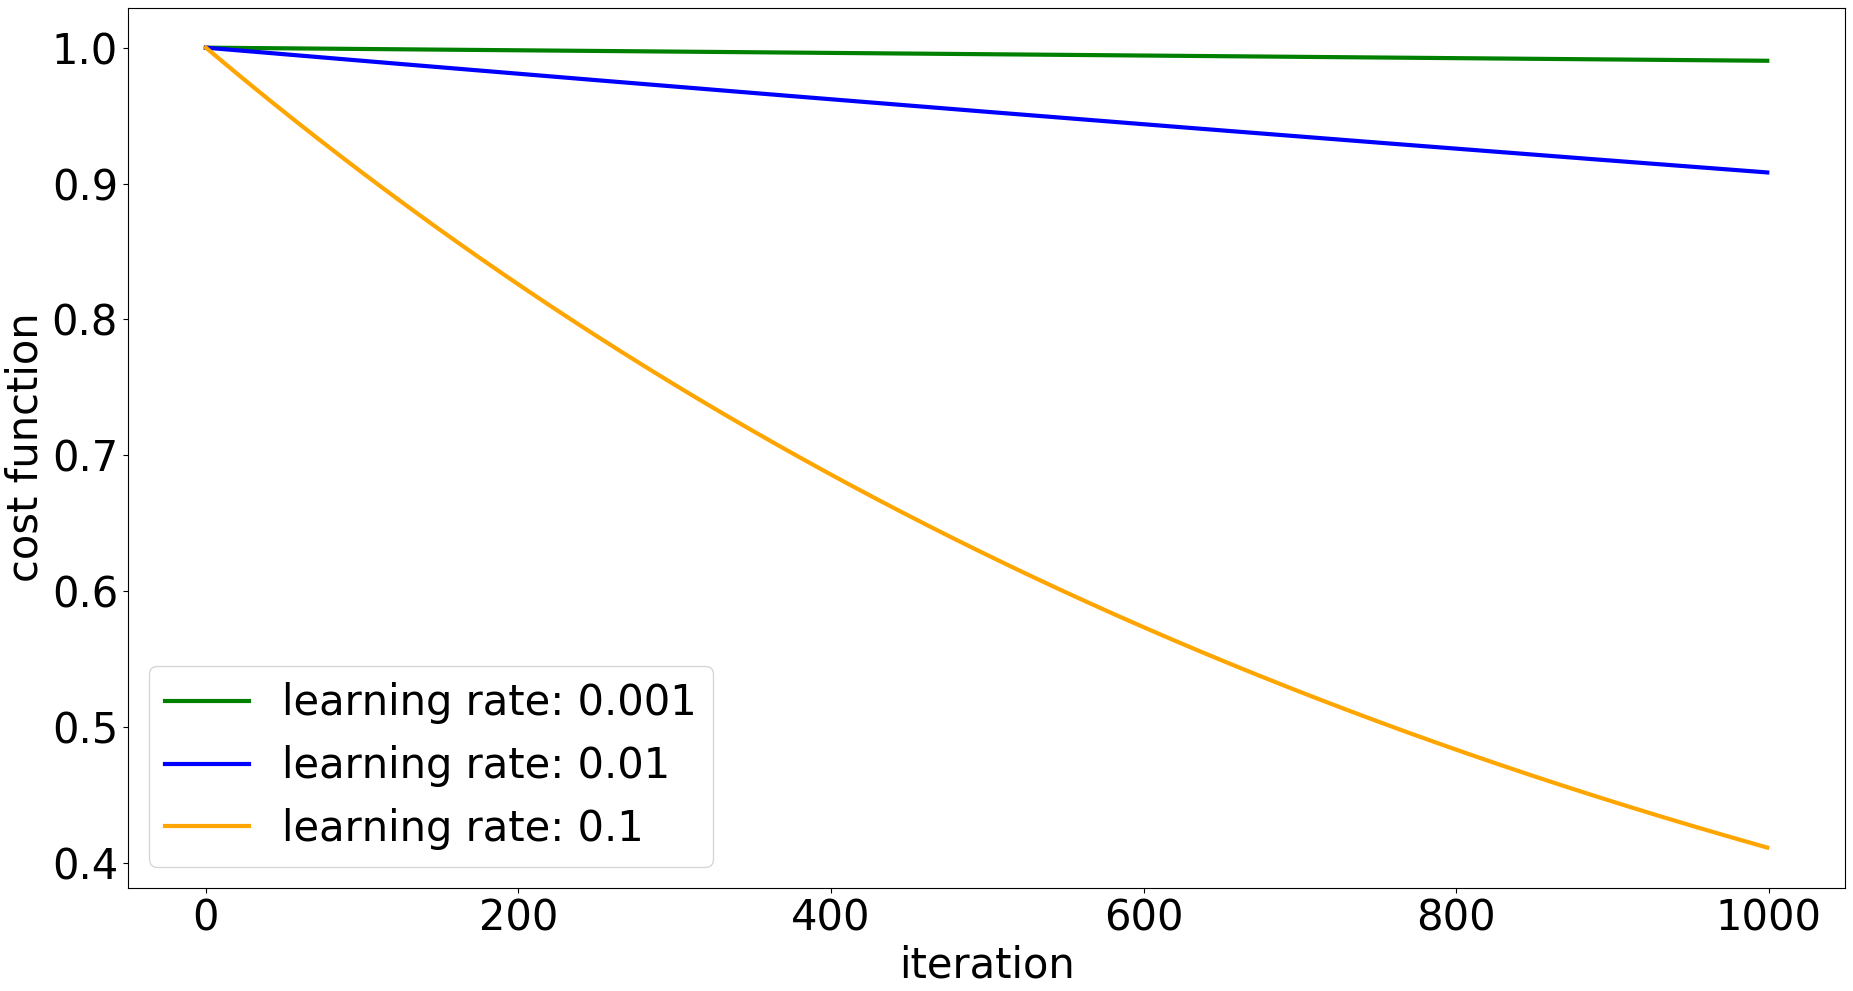
\includegraphics[scale=0.23]{Figure_1.png}

\subsection*{ii.}
After training the linear regression model we obtain the following coefficients:
$\theta_{0} = -2.5002977321421088e-17$, $\theta_{1} = 0.8797086791404171$. 
This gives us the linear model:
\begin{equation*}
    h_{\theta}(x) = \theta_{0} + \theta_{1}x \approx 0 + 0.8797 * x \approx 0.8797x
\end{equation*}

\subsection*{iii.}
I chose the mean $\mu$ as the constant value of the baseline model.
We obtain the following results:

Baseline model:
\begin{equation*}
    J(\theta_{0}, \theta_{1}) = \frac{1}{m}\sum_{i=1}^{m}(h_{\theta}(x^{(i)}) - y^{(i)})^{2} = 0.9999999999999989 \approx 1
\end{equation*}

Trained model:
\begin{equation*}
    J(\theta_{0}, \theta_{1}) = 0.4123744218292116 \approx 0.4124
\end{equation*}

Our goal is to minimise the cost function $J(\theta_{0}, \theta_{1})$. In this case we notice that there is 
a considerable difference between both values of approximately $0.5876$ (note that values are standardised).

\subsection*{iv.}
Using a linear regression model with sklearn, we obtain the following values:

\begin{equation*}
    h_{\theta}(x) = 0.00648141 + 0.94980041x \approx 0.0065 + 0.9498x
\end{equation*}
The cost function for this model is:

\begin{equation*}
    J(\theta_{0}, \theta_{1}) = 0.11706807 \approx 0.1171
\end{equation*}

Remember the cost function for our previous model gave us a value of $J(\theta_{0}, \theta_{1}) \approx 0.4124$
The difference in precision is of $0.29533$. We can conclude that the sklearn trained model
is a much more accurate model (once again, values are standardised).

\section*{Appendix}
Util functions file:
\begin{lstlisting}[language=Python]
import math


def h(coef1, coef2, feature):
    # Returns the value for the model with provided coefs and feature
    return coef1 + coef2 * feature


def get_median(value):
    median = 0
    length = len(value)
    for i in range(length):
        median += value[i][0]
    return median / length


def cost_function(x, y, coef1, coef2):
    # Computes the sum part for the gradient descent algorithm
    length = len(x)
    current_sum = 0
    for i in range(length):
        tmp = h(coef1, coef2, x[i][0]) - y[i][0]
        tmp = tmp * tmp
        current_sum += tmp
    return current_sum / length


def scaling_factor(value):
    # Compute the scaling factor for data standardisation
    # In this case the scaling factor is the std deviation
    length = len(value)
    valsSum = 0
    median = get_median(value)
    for i in range(length):
        valsSum += ((value[i][0] - median) ** 2) / length
    return math.sqrt(valsSum)


def gradient_descent(x, y, rate, iterations):
    # Find coefs that minimize our cost function using gradient descent
    coef1 = 0
    coef2 = 0
    length = len(x)
    deltas = []
    for _ in range(iterations):
        deltas.append(cost_function(x, y, coef1, coef2))
        sum1 = gradient_descent_sum(x, y, coef1, coef2, False)
        sum2 = gradient_descent_sum(x, y, coef1, coef2, True)
        gamma1 = ((-2 * rate) / length) * sum1
        gamma2 = ((-2 * rate) / length) * sum2
        coef1 += gamma1
        coef2 += gamma2
    return {
        "coef_1": coef1,
        "coef_2": coef2,
        "deltas": deltas,
    }


def gradient_descent_sum(x, y, coef1, coef2, multiply):
    # Computes the sum part for the gradient descent algorithm
    length = len(x)
    current_sum = 0
    for i in range(length):
        tmp = h(coef1, coef2, x[i][0]) - y[i][0]
        if multiply == True:
            tmp = tmp * x[i][0]
        current_sum += tmp
    return current_sum / length    
\end{lstlisting}

Main code file:
\begin{lstlisting}[language=Python]
import matplotlib.pyplot as plt
import numpy as np
import pandas as pd
import math
from util import get_median, scaling_factor, cost_function, gradient_descent
from sklearn.linear_model import LinearRegression
from sklearn import preprocessing

# Read data from CSV
df = pd.read_csv("dataset.csv", comment='#')
# Extract columns from data
x = np.array(df.iloc[:, 0])
x = x.reshape(-1, 1)
y = np.array(df.iloc[:, 1])
y = y.reshape(-1, 1)
# Convert x to floats
x = x.astype(float)

# normalise x data
median = get_median(x)
scaling = scaling_factor(x)
length = len(x)
for i in range(length):
    value = x[i][0]
    normalised = (value - median) / scaling
    x[i][0] = normalised

# normalise y data
median = get_median(y)
scaling = scaling_factor(y)
length = len(y)
for i in range(length):
    value = y[i][0]
    normalised = (value - median) / scaling
    y[i][0] = normalised

# For Q1 use 200 iterations and 0.1 learning rates
nb_iterations = 200
coefs = gradient_descent(x, y, 0.1, nb_iterations)

print("Q1, coefficients: ", coefs["coef_1"], coefs["coef_2"])

# Q2 i: use gradient descent on learning rates 0.1, 0.01, 0.001.
nb_iterations = 1000
xaxis = range(nb_iterations)
coefs_001 = gradient_descent(x, y, 0.001, nb_iterations)
coefs_01 = gradient_descent(x, y, 0.01, nb_iterations)
coefs_1 = gradient_descent(x, y, 0.1, nb_iterations)

# Plot the cost function evolution
plt.rc('font', size=30)
plt.rcParams['figure.constrained_layout.use'] = True
plt.plot(xaxis, coefs_001["deltas"], color='green', linewidth=3)
plt.plot(xaxis, coefs_01["deltas"], color='blue', linewidth=3)
plt.plot(xaxis, coefs_1["deltas"], color='orange', linewidth=3)
plt.xlabel("iteration")
plt.ylabel("cost function")
plt.legend(["learning rate: 0.001", "learning rate: 0.01", "learning rate: 0.1"])
# Plot is shown at the end of program executiong as it blocks execution otherwise.

# Q2 ii: use learning rate of 0.5
coefs_05 = gradient_descent(x, y, 0.5, nb_iterations)

print("Q2 ii parameter values after training: ",
      coefs_05["coef_1"], coefs_05["coef_2"])

print("Q2 iii cost function for trained model: ", coefs_05["deltas"][199])
print("Q2 iii cost function for baseline model (using mean): ",
      cost_function(x, y, get_median(y), 0))

# Q3, reload values from dataset to start over
# Read data from CSV
df = pd.read_csv("dataset.csv", comment='#')
# Extract columns from data
x = np.array(df.iloc[:, 0])
x = x.reshape(-1, 1)
y = np.array(df.iloc[:, 1])
y = y.reshape(-1, 1)
# Convert x to floats
x = x.astype(float)

# Standardise data x and y.
x = preprocessing.scale(x)
y = preprocessing.scale(y)

# Separate features into training / test sets.
Xtrain = x[:-20]
Xtest = x[-20:]

# Separate targets as well.
Ytrain = y[:-20]
Ytest = y[-20:]

# Train the model
regr = LinearRegression()
regr.fit(Xtrain, Ytrain)

# Predict using the test set
y_pred = regr.predict(Xtest)

# Print coefficients and cost function output.
print("Q3")
print('Sklearn model Coefficients: ', regr.coef_, regr.intercept_)
print('Sklearn model Cost function: ',
      cost_function(x, y, regr.intercept_, regr.coef_))


# Show plot for Q2 i.
plt.show()
\end{lstlisting}
\end{document}
